\section{Results}

This is the results section.

\begin{align}
	F &= ma \\
	\intertext{where:}
	F &= \text{net force applied on the body [N]} \nonumber \\
	m &= \text{total mass of the body [kg]} \nonumber \\
	a &= \text{net acceleration of the body [m s}^{-2}\text{]} \nonumber
\end{align}

\begin{figure}[htbp!]
	\begin{center}
		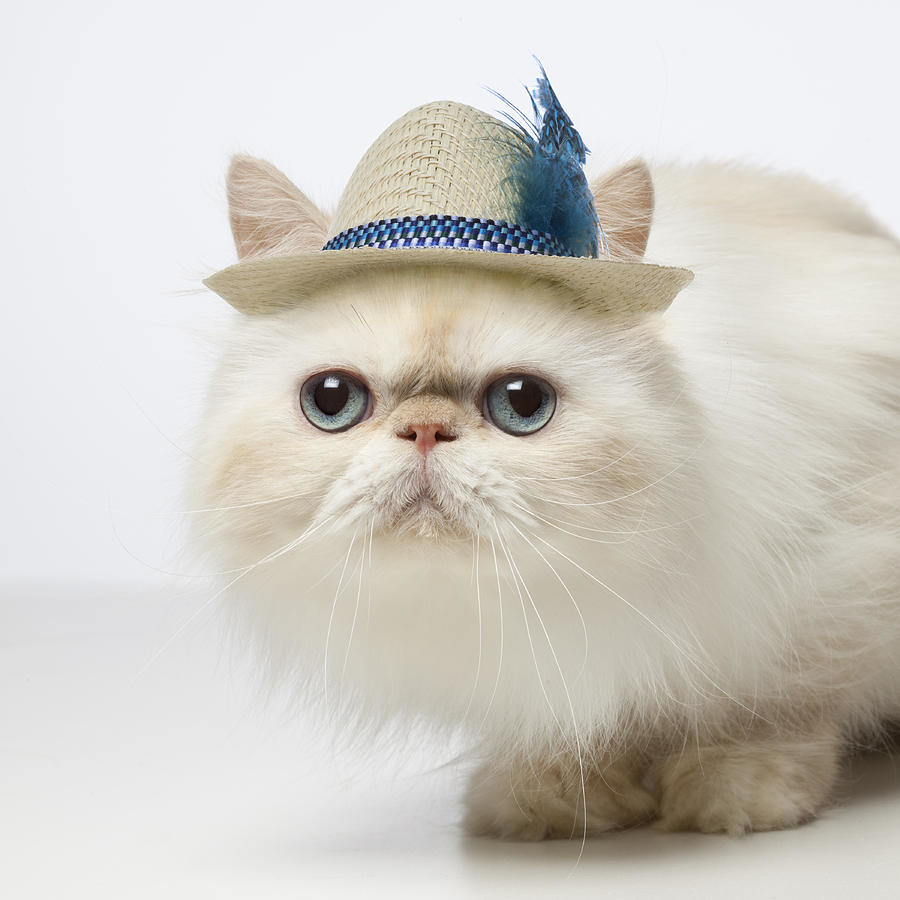
\includegraphics[scale=0.7]{./images/catinhat}
	\end{center}
	\caption{A caption for the figure.}
	\label{fig:catinhat}
\end{figure}

\begin{table}[ht]
	\centering
        \caption{A caption for the table.}
\begin{tabular}{lr}
	\hline
	\textbf{Properties} & \textbf{Value} \\
	\hline
    Mass [kg] & 2,324 \\
    Height [m] & 558 \\
    Volume [m$^3$] & 4,072 \\
    \hline
\end{tabular}
\label{tab:table1}
\end {table}
